%%%%%%%%%%%%%%%%%%%%%%%%%%%%%%%%%%%%%%%%%%%%%%%%%%%%%%%%%%%%%%%%%%%%%%%%%%%%%%%
%
%    NEPI, a framework to manage network experiments
%    Copyright (C) 2013 INRIA
%
%    This program is free software: you can redistribute it and/or modify
%    it under the terms of the GNU General Public License as published by
%    the Free Software Foundation, either version 3 of the License, or
%    (at your option) any later version.
%
%    This program is distributed in the hope that it will be useful,
%    but WITHOUT ANY WARRANTY; without even the implied warranty of
%    MERCHANTABILITY or FITNESS FOR A PARTICULAR PURPOSE.  See the
%    GNU General Public License for more details.
%
%    You should have received a copy of the GNU General Public License
%    along with this program.  If not, see <http://www.gnu.org/licenses/>.
%
% Author: Alina Quereilhac <alina.quereilhac@inria.fr>
%
%%%%%%%%%%%%%%%%%%%%%%%%%%%%%%%%%%%%%%%%%%%%%%%%%%%%%%%%%%%%%%%%%%%%%%%%%%%%%%%


%\documentclass[12pt, openright,twoside]{memoir}
%% avoid blank page between chapters with openany
\documentclass[12pt,openany]{memoir}
%% Make margings on even and odd pages equal
\setulmarginsandblock{3cm}{3cm}{*}
\setlrmarginsandblock{3cm}{3cm}{*}
\checkandfixthelayout

\usepackage[T1]{fontenc}
\usepackage{kpfonts}
\setSingleSpace{1.1}
\SingleSpacing
\usepackage{xcolor,calc}
\definecolor{chaptercolor}{gray}{0.8}

% helper macros
\newcommand\numlifter[1]{\raisebox{-2cm}[0pt][0pt]{\smash{#1}}}
\newcommand\numindent{\kern37pt}
\newlength\chaptertitleboxheight

\makechapterstyle{hansen}{
   \renewcommand\printchaptername{\raggedleft}
    \renewcommand\printchapternum{%
        \begingroup%
        \leavevmode%
        \chapnumfont%
        \strut%
        \numlifter{\thechapter}%
        \numindent%
        \endgroup%
    }
    \renewcommand*{\printchapternonum}{%
        \vphantom{\begingroup%
            \leavevmode%
            \chapnumfont%
            \numlifter{\vphantom{9}}%
            \numindent%
        \endgroup}
    \afterchapternum}
   \setlength\midchapskip{0pt}
   \setlength\beforechapskip{0.5\baselineskip}
    \setlength{\afterchapskip}{3\baselineskip}
    \renewcommand\chapnumfont{%
        \fontsize{4cm}{0cm}%
        \bfseries%
        \sffamily%
        \color{chaptercolor}%
    }
    \renewcommand\chaptitlefont{%
        \normalfont%
        \huge%
        \bfseries%
        \raggedleft%
    }%
    \settototalheight\chaptertitleboxheight{%
    \parbox{\textwidth}{\chaptitlefont \strut bg\\bg\strut}}
    \renewcommand\printchaptertitle[1]{%
        \parbox[t][\chaptertitleboxheight][t]{\textwidth}{%
            %\microtypesetup{protrusion=false}% add this if you use microtype
        \chaptitlefont\strut ##1\strut}%
    }
}
\chapterstyle{hansen}

\usepackage{verbatim}
\usepackage{hyperref}
%% Remove red squares on top of hyperlinks
\hypersetup{%
        pdfborder = {0 0 0}
    }

\usepackage{graphicx}
\usepackage{listings}
\usepackage{color}
\usepackage[scaled]{beramono}

\definecolor{mygreen}{rgb}{0,0.6,0}
\definecolor{mygray}{rgb}{0.5,0.5,0.5}
\definecolor{mymauve}{rgb}{0.58,0,0.82}
\definecolor{mylightgray}{gray}{0.95}

\lstset{ %
  backgroundcolor=\color{mylightgray},   % choose the background color; you must add \usepackage{color} or \usepackage{xcolor}
  basicstyle=\footnotesize\ttfamily,        % the size of the fonts that are used for the code
  breakatwhitespace=false,         % sets if automatic breaks should only happen at whitespace
  breaklines=true,                 % sets automatic line breaking
  captionpos=b,                    % sets the caption-position to bottom
  commentstyle=\color{mygreen},    % comment style
  deletekeywords={...},            % if you want to delete keywords from the given language
  escapeinside={\%*}{*)},          % if you want to add LaTeX within your code
  extendedchars=true,              % lets you use non-ASCII characters; for 8-bits encodings only, does not work with UTF-8
  %frame=single,                    % adds a frame around the code
  keepspaces=true,                 % keeps spaces in text, useful for keeping indentation of code (possibly needs columns=flexible)
  keywordstyle=\color{blue},       % keyword style
  language=Python,                 % the language of the code
  morekeywords={*,...},            % if you want to add more keywords to the set
  %numbers=left,                    % where to put the line-numbers; possible values are (none, left, right)
  %numbersep=5pt,                   % how far the line-numbers are from the code
  %numberstyle=\tiny\color{mygray}, % the style that is used for the line-numbers
  %stepnumber=1,                    % the step between two line-numbers. If it's 1, each line will be numbered
  rulecolor=\color{black},         % if not set, the frame-color may be changed on line-breaks within not-black text (e.g. comments (green here))
  showspaces=false,                % show spaces everywhere adding particular underscores; it overrides 'showstringspaces'
  showstringspaces=false,          % underline spaces within strings only
  showtabs=false,                  % show tabs within strings adding particular underscores
  stringstyle=\color{mymauve},     % string literal style
  tabsize=2,                       % sets default tabsize to 2 spaces
  title=\lstname                   % show the filename of files included with \lstinputlisting; also try caption instead of title
}

\title{NEPI v3.0 User Manual}
\date{}
\author{}
\renewcommand{\maketitlehookd}{%
  \begin{center}
    
\includegraphics[width=6cm]{nepi_logo.png}
\end{center}}

\begin{document}

% clear numbering from first page
\clearpage\maketitle
\thispagestyle{empty}

\pagebreak
\tableofcontents

\chapter{FAQ}
\label{faq}
%%%%%%%%%%%%%%%%%%%%%%%%%%%%%%%%%%%%%%%%%%%%%%%%%%%%%%%%%%%%%%%%%%%%%%%%%%%%%%%
%
%    NEPI, a framework to manage network experiments
%    Copyright (C) 2013 INRIA
%
%    This program is free software: you can redistribute it and/or modify
%    it under the terms of the GNU General Public License as published by
%    the Free Software Foundation, either version 3 of the License, or
%    (at your option) any later version.
%
%    This program is distributed in the hope that it will be useful,
%    but WITHOUT ANY WARRANTY; without even the implied warranty of
%    MERCHANTABILITY or FITNESS FOR A PARTICULAR PURPOSE.  See the
%    GNU General Public License for more details.
%
%    You should have received a copy of the GNU General Public License
%    along with this program.  If not, see <http://www.gnu.org/licenses/>.
%
% Author: Alina Quereilhac <alina.quereilhac@inria.fr>
%
%%%%%%%%%%%%%%%%%%%%%%%%%%%%%%%%%%%%%%%%%%%%%%%%%%%%%%%%%%%%%%%%%%%%%%%%%%%%%%%

\section{What is NEPI?}

NEPI is not a network simulator, nor an emulator or a testbed. 
NEPI is a Python library that provides classes to describe and 
run network experiments on different experimentation platforms
(e.g. Planetlab, OMF wireless testbeds, network simulators, etc).

Imagine that you want to run an experiment to test a distributed 
application you just coded, on the Internet. 
You can use NEPI to deploy your application on PlanetLab
nodes, run the experiment, and collect result files
you might have generated during the
experiment (e.g. pcap files from tcpudmps).

Sure, you could do this by coding your own BASH script, but 
it will probably take more time and painful hours of debugging
if you want to do it right.
NEPI aims at providing a re-usable code base to run network 
experiments on target experimentation platforms, so to 
decrease the time  you spend in developing platform specific 
scripts or programs, and debugging them. 

In a nut-shell, NEPI is a network experiment 
management framework which provides a simple way of 
describing network experiments, and the logic to automatically
deploy those experiments on the target experimentation environments.
It also provides the means to control the resources used in the experiment
(e.g. Nodes, applications, switches, virtual machines, routing table entries, 
etc ) during experiment execution, and to collect results generated by
the experiment to a local repository.

The experiment deployment and control is done by the
Experiment Controller (EC) entity, which is responsible for the 
global orchestration of the experiment. 
The EC knows nothing about how to manage specific resources 
(e.g. how to configure a network interface in a PlanetLab node),
instead it delegates those tasks to entities called Resource Manager (RM).

The RMs are responsible of controlling single resources 
(e.g. a Linux host, an Open vSwitched on PlanetLab 
nodes, etc). Different types of resources will be controlled by
different RMs, specifically adpated to control them.
All RMs implement a same external interface, that the EC uses 
to control them in a uniform way.

NEPI is not magical, it can not control all existing resources
on all existing experimentation platforms by default.
However, potentially any resource could be controlled by 
NEPI if the adequate Resource Manager is implemented for it.
Fortunately, NEPI already provides several Resource Managers for
different resources on a variety of testbeds, and new 
Resource Manager classes can be extended from existing ones,
to control new types of resources. 

The idea behind NEPI is to enable runing network experiments on 
potentially any experimentation platform, using a single
software tool, as opposite to using a dedicated software for 
each platform. An additional perk is that you don't have to deal 
with a lot of platform-specific gory details of setting up and 
configuring the resources (e.g. Creating a TAP device on Planetlab.
If you ever had to do that, you know what I mean). Also, 
you could combine resources from different platforms in a same
experiment, using just one script.

So, 'One ring to rule them all', sorry I meant, 'One tool to 
control them all'... or something like that.
We though it was a good idea to abstract platform details
behind a common resource management interface, and let 
NEPI deal with the details and give you back the results.

\section{What does a NEPI script look like ?}
\label{faq:ping_example}

Here is a very simple experiment example, which runs a PING
to "nepi.inria.fr" from a given host.
Note that you will need to replace the hostname, username, and
ssh\_key variables va to run the example. 

\begin{lstlisting}[language=Python]
from nepi.execution.ec import ExperimentController

ec = ExperimentController(exp_id = "myexperiment")

hostname = # Host that can be accessed with an SSH account
username = # SSH user account on host
ssh_key = # Path to SSH public key file to access host

node = ec.register_resource("linux::Node")
ec.set(node, "hostname", hostname)
ec.set(node, "username", username)
ec.set(node, "identity", ssh_key)

app = ec.register_resource("linux::Application")
ec.set(app, "command", "ping -c3 nepi.inria.fr")
ec.register_connection(app, node)

ec.deploy()

ec.wait_finished(app)

print ec.trace(app, "stdout")

ec.shutdown()

\end{lstlisting}

\section{What does NEPI stands for?}

It stands for: Network Experiment Programming Interface.

\section{Who developed NEPI?}

NEPI was developed at INRIA, Sophia Antipolis France.
A first prototype was implemented in 2010. 
Versions 1.0 and 2.0 were released in 2011 and 2012, respectively. 
The current version is 3.0, and it was completely redesigned and
rewritten to broaden the scope, and to include several  
new features, which will be described in detail in this document.
The following people has contributed to the project:

\begin{itemize}
  \item NEPI version 3.0: Alina Quereilhac, Julien Tribino, Lucia Guevgeozian Odizzio, Alexandros Kouvakas
  \item NEPI versions 1.0 and 2.0: Alina Quereilhac, Claudio Freire, Martin Ferrari, Mathieu Lacage
  \item NEPI prototype: Martin Ferrari, Mathieu Lacage
  \item Other contributors: Dirk Hasselbalch
\end{itemize}

\section{Is it free?}

Yes, NEPI is free software. It is free to use, free to modify, free to share.
NEPI v3.0 is licensed under GPL v3, so you can do whatever you want with it, 
as long as you keep the same license. 

\section{How can I contribute?}

There are many ways you can contribute to the project. 
The first one is using it and reporting bugs. 
You can report bugs on the NEPI bugzilla page at: 

\url{http://nepi.inria.fr/bugzilla} \\

You can also become a part of the NEPI community and join our mailing lists:

\begin{itemize}
    \item To subscribe to the users mailing list at \textit{nepi-users@inria.fr}
        you can send an email to \textit{sympa@inria.fr} with subject
        \textit{Subscribe nepi-users <put-your-user-name-here>}
    \item To subscribe to the developers mailing list at \textit{nepi-developers@inria.fr}
        you can send an email to \textit{sympa@inria.fr} with subject
        \textit{Subscribe nepi-developers <put-your-user-name-here>}
    \end{itemize}

To contribute with bug fixes and new features, please send your code patch
to the \textit{nepi-developers} list.

\section{How can I report a bug ?}

To report a bug take a look at the NEPI bugzilla page at :

\url{http://nepi.inria.fr/bugzilla} \\

\section{Where can I get more information ?}

For more information visit NEPI web site at :

\url{http://nepi.inria.fr} \\




\chapter{Getting started}
\label{getting_started}
%%%%%%%%%%%%%%%%%%%%%%%%%%%%%%%%%%%%%%%%%%%%%%%%%%%%%%%%%%%%%%%%%%%%%%%%%%%%%%%
%
%    NEPI, a framework to manage network experiments
%    Copyright (C) 2013 INRIA
%
%    This program is free software: you can redistribute it and/or modify
%    it under the terms of the GNU General Public License as published by
%    the Free Software Foundation, either version 3 of the License, or
%    (at your option) any later version.
%
%    This program is distributed in the hope that it will be useful,
%    but WITHOUT ANY WARRANTY; without even the implied warranty of
%    MERCHANTABILITY or FITNESS FOR A PARTICULAR PURPOSE.  See the
%    GNU General Public License for more details.
%
%    You should have received a copy of the GNU General Public License
%    along with this program.  If not, see <http://www.gnu.org/licenses/>.
%
% Author: Alina Quereilhac <alina.quereilhac@inria.fr>
%
%%%%%%%%%%%%%%%%%%%%%%%%%%%%%%%%%%%%%%%%%%%%%%%%%%%%%%%%%%%%%%%%%%%%%%%%%%%%%%%

NEPI is written in Python, so you will need to install Python before 
being able to run experiments with NEPI. 
NEPI is known to work on Linux (Fedore, Debian, Ubuntu) and Mac (OS X).

\section{Dependencies}

Dependencies for NEPI vary according to the features you want to enable.
Make sure the following dependencies are correctly installed in your system
before using NEPI. \\

Mandatory dependencies:
\begin{itemize}
    \item Python 2.6+
    \item Mercurial
    \item python-ipaddr
    \item python-networkx
    \item python-pygraphviz
    \item python-matplotlib 
\end{itemize}

Optional dependencies:
\begin{itemize}
    \item SleekXMPP - Required to run experiments on OMF testbeds
\end{itemize}

\subsection{Install dependencies on Debian/Ubuntu}

\begingroup
    \fontsize{10pt}{12pt}\selectfont

\begin{verbatim}
    $ sudo apt-get -y install python mercurial python-ipaddr python-networkx python-pygraphviz python-matplotlib
\end{verbatim}

\endgroup

\subsection{Install dependencies on Fedora}

\begingroup
    \fontsize{10pt}{12pt}\selectfont

\begin{verbatim}
    $ sudo yum -y install python mercurial python-ipaddr python-networkx graphviz-python python-matplotlib
\end{verbatim}

\endgroup

\subsection{Install dependencies on Mac}

First install homebrew (\url{http://mxcl.github.io/homebrew/}),
then you can install Python and the rest of the dependencies as follows:

\begingroup
    \fontsize{10pt}{12pt}\selectfont

\begin{verbatim}
   $ brew install python
   $ sudo port install mercurial
   $ sudo easy_install pip
   $ sudo pip install ipaddr
   $ sudo pip install networkx
   $ sudo  pip install pygraphviz
   $ sudo  pip install matplotlib
\end{verbatim}

\endgroup

To use Python you will need to set the PATH environmental variable as:

\begingroup
    \fontsize{10pt}{12pt}\selectfont

\begin{verbatim}
   $ export PATH=$PATH:/usr/local/share/python
\end{verbatim}

\endgroup

\subsection{Install SleekXMPP}

You will need \textit{git} to get the SleekXMPP sources.

\begingroup
    \fontsize{10pt}{12pt}\selectfont

\begin{verbatim}
    $ git clone -b develop git://github.com/fritzy/SleekXMPP.git
    $ cd SleekXMPP
    $ sudo python setup.py install
\end{verbatim}

\endgroup

\section{The source code}

To get NEPI's source code you will need Mercurial version 
control system. The Mercurial NEPI repo can also be browsed online at: \\

\url{http://nepi.inria.fr/code/nepi/} 

\subsection{Clone the repo}

\begingroup
    \fontsize{10pt}{12pt}\selectfont

\begin{verbatim}
$ hg clone http://nepi.inria.fr/code/nepi -r nepi-3-dev
\end{verbatim}

\endgroup

\section{Install NEPI in your system}

You don't need to install NEPI in your system to be able to run 
experiments. However this might be convenient if you don't 
plan to modify or extend the sources.

To install NEPI, just run \emph{make install} in the NEPI source
folder.

\begingroup
    \fontsize{10pt}{12pt}\selectfont

\begin{verbatim}
    $ cd nepi
    $ make install 
\end{verbatim}

\endgroup

If you are developing your own NEPI extensions, the installed 
NEPI version might interfere with your work.
In this case it is probably more convenient to tell
Python where to find the NEPI sources, using the PYTHONPATH
environmental variable, when you run a NEPI script.

\begingroup
    \fontsize{10pt}{12pt}\selectfont

\begin{verbatim}
    $ export PYTHONPATH=$PYTHONPATH:<path-to-nepi>/src 
\end{verbatim}

\endgroup

\section{Run experiments}

There are two ways you can use NEPI to run your experiments.
The first one is writing a Python script, which will import
NEPI libraries, and run it. 
The second one is in interactive mode by using Python console.

\subsection{Run from script}

Writing a simple NEPI expeiment script is easy.
Take a look at the example in the FAQ section \ref{faq:ping_example}.
Once you have written down the script, you can run it using
Python. If NEPI is not installed in your system,
you will need to export the path to NEPI's source code to 
the PYTHONPATH environment variable, so that Python can find
NEPI's libraries.

\begingroup
    \fontsize{10pt}{12pt}\selectfont

\begin{verbatim}
    $ export PYTHONPATH=<path-to-nepi>/src:$PYTHONPATH
    $ cd <path-to-nepi> 
    $ python examples/linux/ping.py -a localhost
\end{verbatim}

\endgroup

\subsection{Run NEPI interactively}

The IPython console can be used as an interactive interpreter to 
execute Python instructions. We can take advantage of this feature, 
to interactively run NEPI experiments. 
We will use the IPython console for the example below. 

You can easily install IPython on Debian, Ubuntu, Fedora or Mac as follows:\\

\textbf{Debian/Ubuntu}

\begingroup
    \fontsize{10pt}{12pt}\selectfont

\begin{verbatim}
    $ sudo apt-get install ipython
\end{verbatim}

\endgroup

\textbf{Fedora}\\

\begingroup
    \fontsize{10pt}{12pt}\selectfont

\begin{verbatim}
    $ sudo yum install ipython
\end{verbatim}

\endgroup

\textbf{Mac}\\

\begingroup
    \fontsize{10pt}{12pt}\selectfont

\begin{verbatim}
    $ pip install ipython
\end{verbatim}

\endgroup

Before starting, make sure to add Python and IPython source directory 
path to the PYTHONPATH environment variable

\begingroup
    \fontsize{10pt}{12pt}\selectfont

\begin{verbatim}
    $ export PYTHONPATH=$PYTHONPATH:/usr/local/lib/python:/usr/local/share/python/ipython
\end{verbatim}

\endgroup

Then you can start IPython as follows: 

\begin{verbatim}
$ export PYTHONPATH=<path-to-nepi>/src:$PYTHONPATH
$ ipython
Python 2.7.3 (default, Jan  2 2013, 13:56:14) 
Type "copyright", "credits" or "license" for more information.

IPython 0.13.1 -- An enhanced Interactive Python.
?         -> Introduction and overview of IPython's features.
%quickref -> Quick reference.
help      -> Python's own help system.
object?   -> Details about 'object', use 'object??' for extra details.

\end{verbatim}

If you want to paste many lines at once in IPython, you will need 
to type \emph{\%cpaste} and finish the paste block with \emph{\-\-}.

The first thing we need to do to describe an experiment with NEPI 
is to import the NEPI Python modules. 
In particular we need to import the ExperimentController class. 
To do this type the following in the Python console: 

\begin{lstlisting}[language=Python]

from nepi.execution.ec import ExperimentController

\end{lstlisting}

After importing the ExperimentController class, it is possible to 
create a new instance of an the ExperimentController (EC) for 
your experiment. 
The <exp-id> argument is the name you want to give the experiment 
to identify it and distinguish it from other experiments. 

\begin{lstlisting}[language=Python]

ec = ExperimentController(exp_id = "<your-exp-id>")

\end{lstlisting}

Next we will define two Python functions: \emph{add\_node} and \emph{add\_app}.
The first one to register \textit{LinuxNodes} resources and the second one to 
register LinuxApplications resources. 

\begin{lstlisting}[language=Python]

%cpaste
def add_node(ec, hostname, username, ssh_key):
    node = ec.register_resource("linux::Node")
    ec.set(node, "hostname", hostname)
    ec.set(node, "username", username)
    ec.set(node, "identity", ssh_key)
    ec.set(node, "cleanHome", True)
    ec.set(node, "cleanProcesses", True)
    return node

def add_app(ec, command, node):
    app = ec.register_resource("linux::Application")
    ec.set(app, "command", command)
    ec.register_connection(app, node)
    return app
--

\end{lstlisting}

The method \textit{register\_resource} registers a resource instance with the 
ExperimentController. The method \textit{register\_connection} indicates
that two resources will interact during the experiment. 
Note that invoking \textit{add\_node} or \textit{add\_app} has no effect other
than informing the EC about the resources that will be used during the experiment.
The actual deployment of the experiment requires the method \textit{deploy} to
be invoked.

The \textit{LinuxNode} resource exposes the hostname, username and identity 
attributes. This attributes provide information about the SSH credentials 
needed to log in to the Linux host. 
The \textit{hostname} is the one that identifies the physical host you want
to access during the experiment. The \textit{username} must correspond to a
valid account on that host, and the \textit{identity} attribute is the 
'absolute' path to the SSH private key in your local computer that allows you 
to log in to the host.

The \textit{command} attribute of the \textit{LinuxApplication} resource 
expects a BASH command line string to be executed in the remote host.
Apart from the \emph{command} attribute, the \emph{LinuxApplication} 
resource exposes several other attributes that allow to upload, 
compile and install arbitrary sources. 
The add\_app function registers a connection between a \textit{LinuxNode} and a 
\textit{LinuxApplication}. 

Lets now use these functions to describe a simple experiment. 
Choose a host where you have an account, and can access using SSH
key authentication. 

\begin{lstlisting}[language=Python]

hostname = "<the-hostname>"
username = "<my-username>"
identity = "</home/myuser/.ssh/id_rsa>"

node = add_node(ec, hostname, username, ssh_key)
app = add_app(ec, "ping -c3 nepi.inria.fr",  node)

\end{lstlisting}

The values returned by the functions add\_node and add\_app are global 
unique identifiers (guid) of the resources that were registered with the EC. 
The guid is used to reference the ResourceManager associated to a registered
resource (for instance to retrieve results or change attribute values).

Now that we have registered some resources, we can ask the ExperimentController
(EC) to deploy them. 
Invoking the \emph{deploy} command will not only configure the 
resource but also automatically launch the applications.

\begin{lstlisting}[language=Python]

 ec.deploy()

\end{lstlisting}

After some seconds, we should see some output messages informing us about the
progress in the host deployment.
If you now open another terminal and you connect to the host using 
SSH (as indicated below), you should see that a directory for your experiment 
has been created in the host. In the remote host you will see that two NEPI 
directories were created in the \$HOME directory: \emph{nepi-src} and \emph{nepi-exp}. 
The first one is where NEPI will store files that might be re used by many 
experiments (e.g. source code, input files) . The second directory \emph{nepi-exp}, 
is where experiment specific files (e.g. results, deployment scripts) will be stored. 

\begingroup
    \fontsize{10pt}{12pt}\selectfont

\begin{verbatim}

$ ssh -i identity username@hostname

\end{verbatim}

\endgroup

Inside the \emph{nepi-exp} directory, you will find another directory with 
the <exp-id> assigned to your EC, and inside that directory you should find 
one directory named node-1 which will contain the files (e.g. result traces) 
associated to the LinuxNode reosurce you just deployed. 
In fact for every resource deployed associated to that host (e.g. each 
LinuxApplication), NEPI will create a directory to place files related to it. 
The name of the directory identifies the type of resources (e.g. 'node', 
'app', etc) and it is followed by the global unique identifier (guid).

We can see if a resource finished deploying by querying its state through the EC 

\begin{lstlisting}[language=Python]

ec.state(app, hr=True)

\end{lstlisting}

Once a \textit{LinuxApplication} has reached the state 'STARTED', 
we can retrieve the 'stdout' trace, which should contain the output 
of the PING command. 

\begin{lstlisting}[language=Python]

 ec.trace(app, "stdout")

\end{lstlisting}

That is it. We can terminate the experiment by invoking the method \emph{shutdown}.

\begin{lstlisting}[language=Python]

 ec.shutdown()

\end{lstlisting}

\subsection{Define a workflow}

Now that we have introduced to the basics of NEPI, we will register 
two more applications and define a workflow where one application 
will start after the other one has finished executing. 
For this we will use the EC \textit{register\_condition} method described below:

\begin{lstlisting}[language=Python]

register_condition(self, guids1, action, guids2, state, time=None):
    Registers an action START, STOP or DEPLOY for all RM on list
    guids1 to occur at time 'time' after all elements in list guids2 
    have reached state 'state'.
    
        :param guids1: List of guids of RMs subjected to action
        :type guids1: list
    
        :param action: Action to perform (either START, STOP or DEPLOY)
        :type action: ResourceAction
    
        :param guids2: List of guids of RMs to we waited for
        :type guids2: list
    
        :param state: State to wait for on RMs of list guids2 (STARTED,
            STOPPED, etc)
        :type state: ResourceState
    
        :param time: Time to wait after guids2 has reached status 
        :type time: string

\end{lstlisting}

To use the \textit{register\_condition} method we will need to import the 
ResourceState and the ResourceAction classes

\begin{lstlisting}[language=Python]

from nepi.execution.resource import ResourceState, ResourceAction

\end{lstlisting}

Then, we register the two applications. The first application will 
wait for 5 seconds and the create a file in the host called "greetings" 
with the content "HELLO WORLD". 
The second application will read the content of the file and output it 
to standard output. If the file doesn't exist il will instead output the 
string "FAILED".

\begin{lstlisting}[language=Python]

app1 = add_app(ec, "sleep 5; echo 'HELLO WORLD!' > ~/greetings", node)
app2 = add_app(ec, "cat ~/greetings || echo 'FAILED'", node)

\end{lstlisting}

In order to guarantee that the second application is successful, we need to 
make sure that the first application is executed first. For this we register 
a condition:

\begin{lstlisting}[language=Python]

ec.register_condition (app2, ResourceAction.START, app1, ResourceState.STOPPED)

\end{lstlisting}

We then deploy the two application:

\begin{lstlisting}[language=Python]

ec.deploy(guids=[app1,app2])

\end{lstlisting}

Finally, we retrieve the standard output of the second application, 
which should return the string "HELLO WORLD!".

\begin{lstlisting}[language=Python]

ec.trace(app2, "stdout")

\end{lstlisting}



\chapter{Introduction to NEPI}
\label{introduction}
%%%%%%%%%%%%%%%%%%%%%%%%%%%%%%%%%%%%%%%%%%%%%%%%%%%%%%%%%%%%%%%%%%%%%%%%%%%%%%%
%
%    NEPI, a framework to manage network experiments
%    Copyright (C) 2013 INRIA
%
%    This program is free software: you can redistribute it and/or modify
%    it under the terms of the GNU General Public License as published by
%    the Free Software Foundation, either version 3 of the License, or
%    (at your option) any later version.
%
%    This program is distributed in the hope that it will be useful,
%    but WITHOUT ANY WARRANTY; without even the implied warranty of
%    MERCHANTABILITY or FITNESS FOR A PARTICULAR PURPOSE.  See the
%    GNU General Public License for more details.
%
%    You should have received a copy of the GNU General Public License
%    along with this program.  If not, see <http://www.gnu.org/licenses/>.
%
% Author: Alina Quereilhac <alina.quereilhac@inria.fr>
%
%%%%%%%%%%%%%%%%%%%%%%%%%%%%%%%%%%%%%%%%%%%%%%%%%%%%%%%%%%%%%%%%%%%%%%%%%%%%%%%

% Motivation
During the past decades, a wide variety of platforms to conduct network
experiments, including simulators, emulators and live testbeds,
have been made available to the research community.
Some of these platforms are tailored for very specific use cases (e.g.
PlanetLab for very realistic Internet application level scenarios), 
while others support more generic ones (e.g. ns-3 for controllable 
and repeatable experimentation). Nevertheless, no single platform is 
able to satisfy all possible scenarios, and so researchers often rely 
on different platforms to evaluate their ideas.

Given the huge diversity of available platforms, it is to be expected a
big disparity in the way to carry out an experiment between one platform and 
another. Indeed, different platforms provide their own mechanisms to 
access resources and different tools to conduct experiments. 
These tools vary widely, for instance, to run a ns-3 simulation it is 
necessary to write a C++ program, while to conduct an experiment using
PlanetLab nodes, one must first provision resources through a special web
service, and then connect to the nodes using SSH to launch any applications
involved in the experiment.

Mastering such diversity of tools can be a daunting task, 
but the complexity of conducting network experiments is not only limited 
to having to master different tools and services.
Designing and implementing the programs and scripts to run an experiment
can be a time consuming and difficult task, specially if distributed
resources need to be synchronised to perform the right action at the
right time. Detecting and handling possible errors during experiment
execution also posses a challenge, even more when dealing with large size
experiments. Additionally, difficulties related to instrumenting the 
experiment and gathering the results must also be considered.

% Challenge
In this context, the challenges that NEPI addresses are manifold. 
Firstly, to simplify the complexity of running network experiments. 
Secondly, to simplify the use of different experimentation platforms, 
allowing to easily switch from one to another. 
Thirdly, to simplify the
use of resources from different platforms at the same time in 
a single experiment.

% How?
The approach proposed by NEPI consists on exposing a generic API
that researchers can use to \emph{program} experiments, and 
providing the libraries that can execute those experiments on 
target network experimentation platforms. The API abstracts the
researchers from the details required to actually run an experiment
on a given platform, while the libraries provide the code to 
automatically perform the steps necessary to deploy the experiment 
and manage resources.

The API is generic enough to allow describing potentially any 
type of experiment, while the architecture of the libraries was 
designed to be extensible to support arbitrary platforms.
A consequence of this is that any new platform can be supported in 
NEPI without changing the API, in a way that is transparent 
to the users.

% 
\section{Experiment Description}

NEPI represents experiments as graphs of interconnected resources.
A resource is an abstraction of any component that takes part of an 
experiment and that can be controlled by NEPI. 
It can be a software or hardware component, it could be a virtual 
machine, a switch, a remote application process, a sensor node, etc.

Resources in NEPI are described by a set of attributes, traces and 
connections. The attributes define the configuration of the resource,
the traces represent the results that can be collected for that resource
during the experiment and the connections represent how a resource relates
to other resources in the experiment.

\begin{figure}[h]
  \centering
  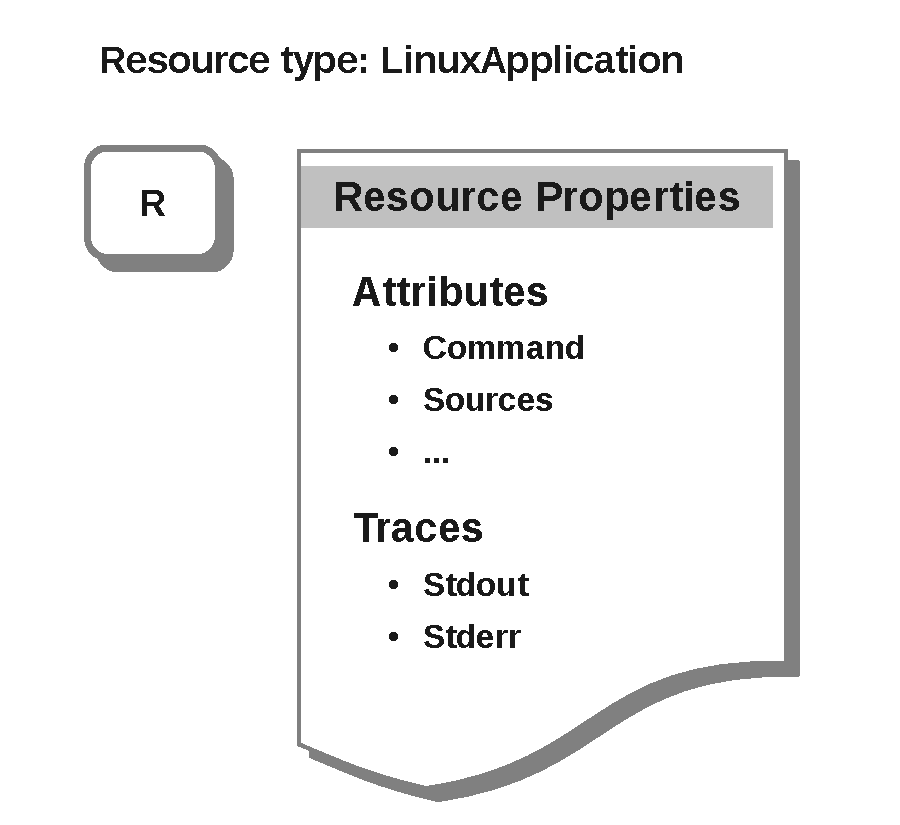
\includegraphics[width=0.5\textwidth]{intro_resource}
  \caption{Properties of a resource of type LinuxApplication}
  \label{fig:intro_resources}
\end{figure}

Examples of attributes are a linux hostname, an IP address to be 
assigned to a network interface, a command to run as a remote application.
Examples of traces are the standard output or standard error of a
running application, a tcpdump on a network interface, etc.

Resources are also associated to a type (e.g. a Linux host, 
a Tap device on PlanetLab, an application running on a Linux host, etc).
Different types of resources expose different attributes and traces
and can be connected to other specific types (e.g. A resource representing
a wireless channel can have an attribute SSID and be connected to a 
Linux interface but not directly to a Linux host resource)
Figure \ref{fig:intro_resources} exemplifies this concept.

There are two different types of connections between resources, the 
first one is used to define the \emph{topology graph} of the experiment.
This graph provides information about which resources will interact
with which other resources during the experiment
(e.g. application A should run in host B, and host B will be connected
to wireless channel D through a network interface C).
Figure \ref{fig:intro_topo_graph} shows a representation of the concept of
topology graph to describe the an experiment.

\begin{figure}[h]
  \centering
  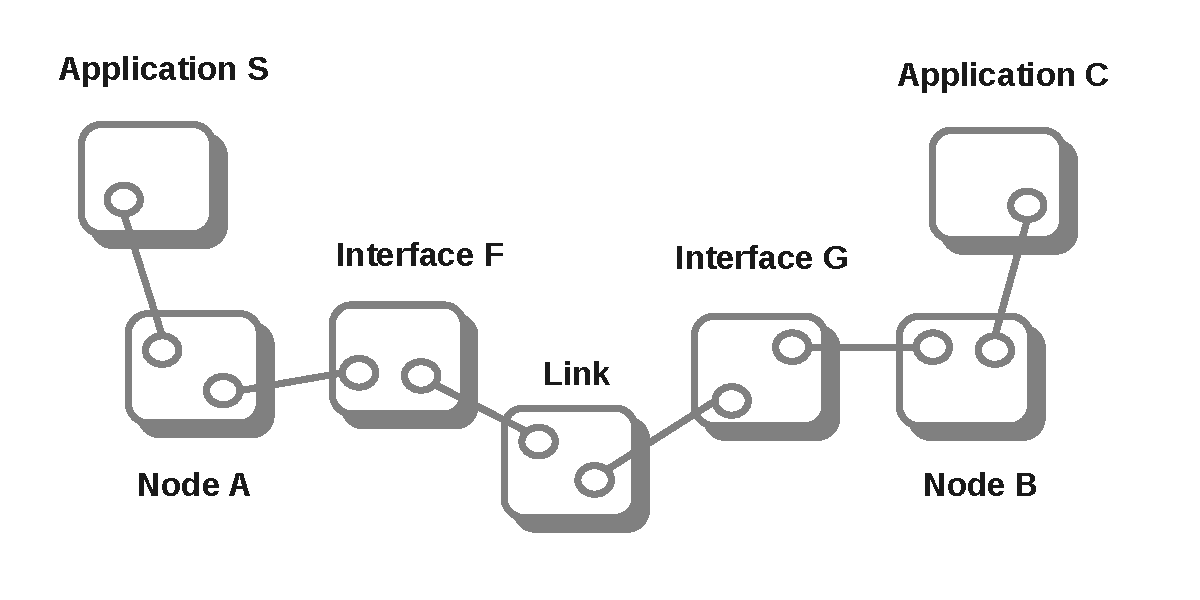
\includegraphics[width=0.8\textwidth]{intro_topo_graph}
  \caption{A topology graph representation of an abstract experiment}
  \label{fig:intro_topo_graph}
\end{figure}

The second type of connections (called conditions to differentiate them 
from the first type) specifies the \emph{dependencies graph}. 
This graph is optional and imposes constraints on the experiment 
workflow, that is the order in which different events occur during the 
experiment. For instance, as depicted in Figure \ref{fig:intro_dependencies_graph}
a condition on the experiment could specify that
a server application has to start before a client application does, or that
an network interface needs to be stopped (go down) at a certain time after
the beginning of the experiment. 

\begin{figure}[h]
  \centering
  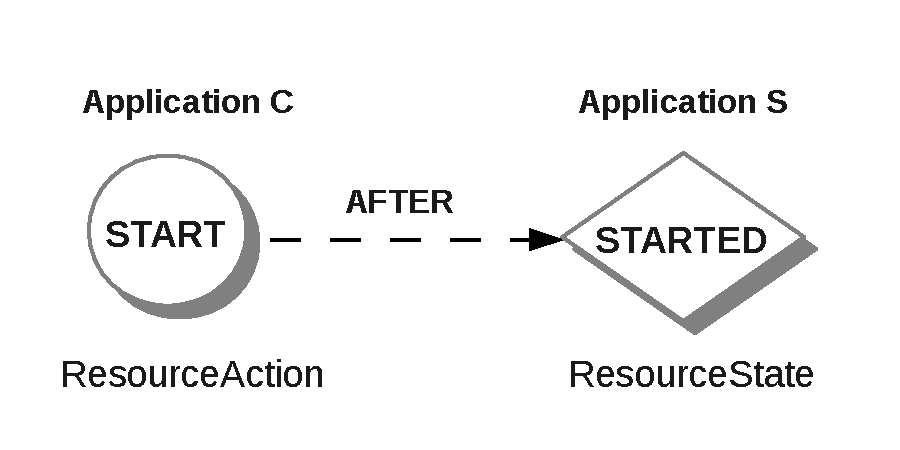
\includegraphics[width=0.8\textwidth]{intro_dependencies_graph}
  \caption{A dependencies graph representation involving two applications 
    resources in an experiment}
  \label{fig:intro_dependencies_graph}
\end{figure}

It is important to note, that the \emph{topology graph} also defines 
implicit and compulsory workflow constraints
(e.g. if an application is \emph{topologically} connected to a host,
the host will always need to be up and running before an application 
can run on it). 
The difference is that the \emph{dependency graph} adds complementary
constraints specified by the user, related to the behavior of the 
experiment.

This technique for modeling experiments is generic enough that can be used 
to describe experiments involving resources from any experimentation 
environment (i.e. testbed, simulator, emulator, etc). However, it
does not provide by itself any information about how to actually deploy
and run an experiment using concrete resources. 


\section{Experiment Life Cycle}

The Experiment Description by itself is not enough to conduct an experiment.
In order to run an experiment it is necessary to translate the description 
into concrete actions and to perform these actions on the specific resources
taking part of the experiment. NEPI does this for the user in an automated
manner.

\begin{figure}[h]
  \centering
  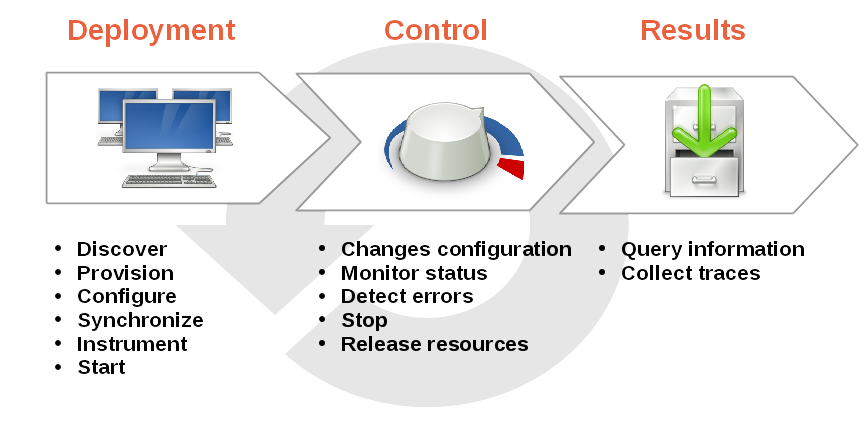
\includegraphics[width=0.8\textwidth]{intro_life_cycle}
  \caption{Common stages of a network experiment life cycle}
  \label{fig:intro_life_cycle}
\end{figure}

Given that different resources will require performing actions in 
different ways (e.g. deploying an application on 
a Linux machine is different than deploying a mobile wireless robot), 
NEPI abstracts the life cycle of resources into common stages associated
to generic actions, and allows to plug-in different implementation of 
these actions for different types of resources.
Figure \ref{fig:intro_life_cycle} shows the three
main stages of the network experiment life cycle, \emph{Deployment}, 
\emph{Control} and \emph{Result (collection)}, and the actions that are 
involved in each of them. 

\begin{figure}[h]
  \centering
  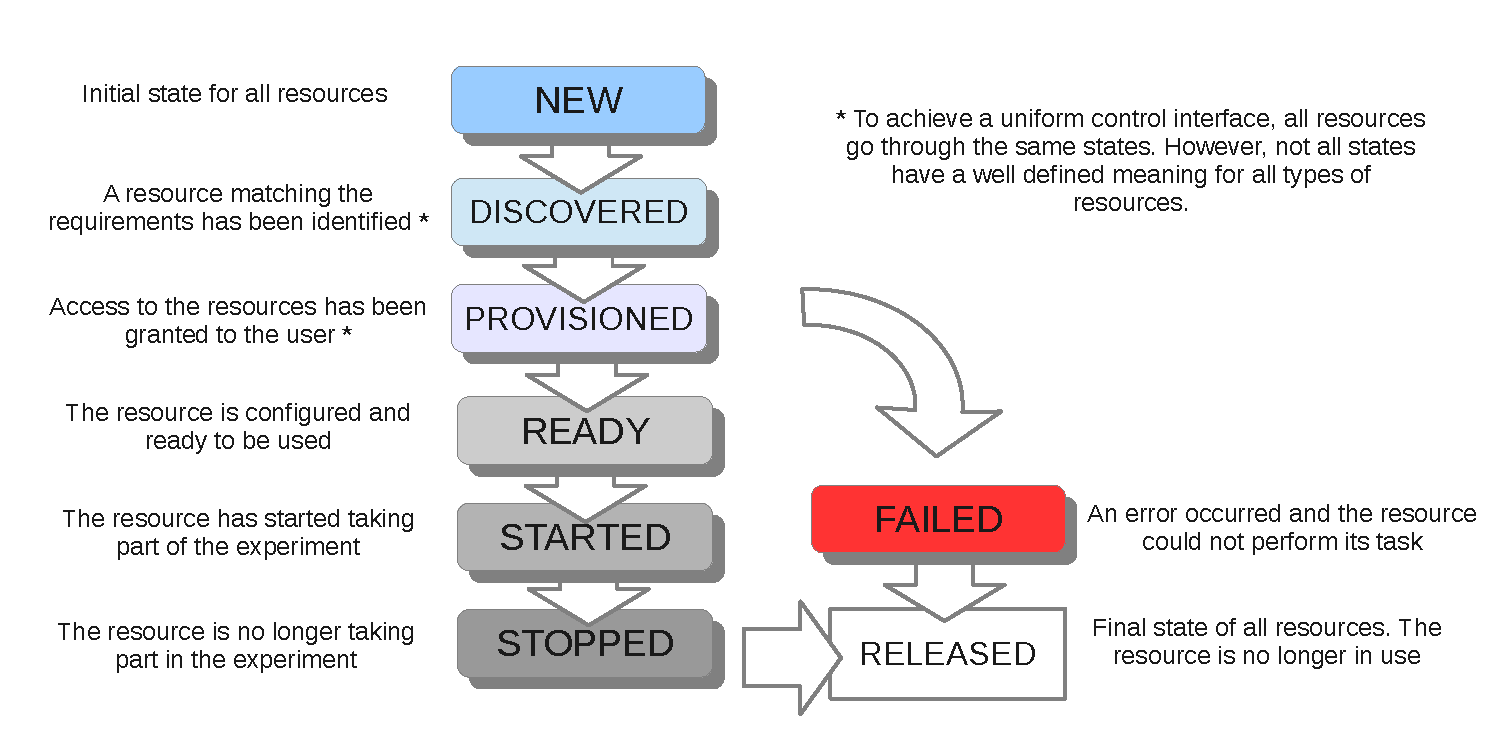
\includegraphics[width=\textwidth]{intro_state_transitions}
  \caption{Resources state transitions}
  \label{fig:intro_state_transitions}
\end{figure}

In order to be able to control different types of resources in 
a uniform way, NEPI assigns a generic state to each of these
actions and expects all resources to follow the same set of
state transitions during the experiment life. The states and
state transitions are depicted in Figure 
\ref{fig:intro_state_transitions}.

It is important to note that NEPI does not require these states
to be globally synchronized for all resources (e.g. resources
are not required to be all ready or started at the same time).
NEPI does not even require all resources to be declared and known 
at the beginning of the experiment, making it possible to use 
an \emph{interactive deployment} mode, where new resources can de 
declared and deployed on the fly, according to the experiment needs.
This interactive mode can be useful to run experiments with the 
purpose of exploring a new technology, or to use NEPI as an adaptive
experimentation tool, that could change an experiment according to
external conditions or measurements. 

\section{Resource Management: The EC \& The RMs}

The Experiment Controller (EC) is the entity that is responsible for 
translating the Experiment Description into a running experiment.
It holds the \emph{topology} and \emph{dependencies} graphs, and it 
exposes a generic experiment control API that the user can 
invoke to deploy experiments, control resources and collect results. 

\begin{figure}[h]
  \centering
  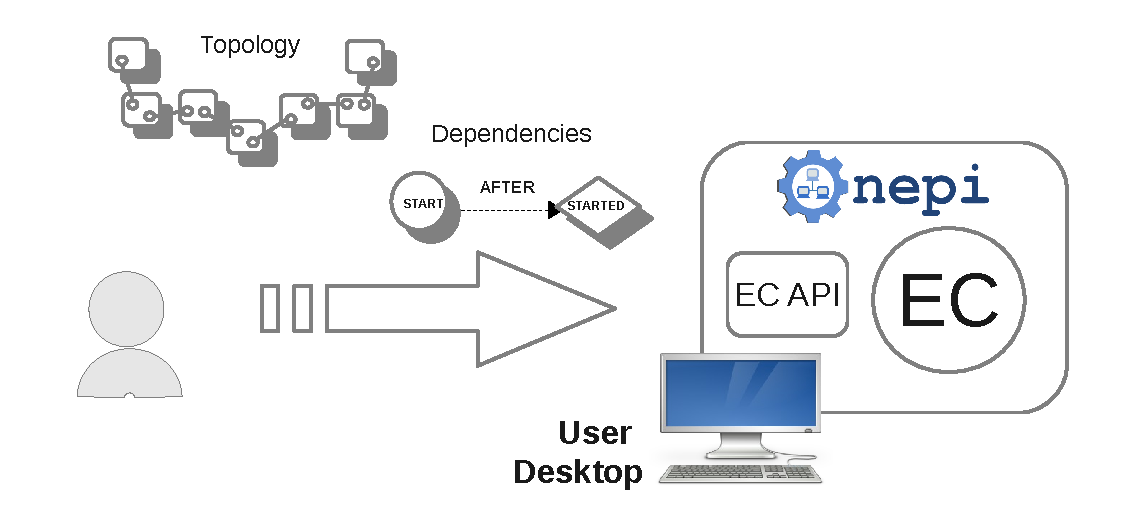
\includegraphics[width=\textwidth]{intro_ec}
  \caption{User interacting with the Experiment Controller}
  \label{fig:intro_ec}
\end{figure}

As shown in Figure \ref{fig:intro_ec}, the user declares the resources and
their dependencies directly with the EC. 
When the user requests the EC to deploy a certain resource or a
group of resources, the EC will take care of performing all the necessary 
actions without further user intervention, including the sequencing of 
actions to respect user defined and topology specific dependencies, 
through internal scheduling mechanisms. 

The EC is a generic entity responsible for the global orchestration of
the experiment. As such, it abstracts itself from the details of how to
control concrete resources and relies on other entities called Resource Managers 
(RM)s to perform resource specific actions. 

For each resource that the user registers in the \emph{topology graph}, the EC
will instantiate a RM of a corresponding type. A RM is a resource specific
controller and different types of resources require different type of
RMs, specifically adapted to manage them.

The EC communicates with the RMs through a well defined API that exposes
the necessary methods (actions) to achieve all the state transitions defined by the
common resource life-cycle. Each type of RM must provide a specific implementation
for each action and ensure that the correct state transition has been achieved
for the resource (e.g. upon invocation of the START action, the RM must take 
the necessary steps to start the resource and set itself to state STARTED).
This decoupling between the EC and the RMs makes it possible to extend the 
control capabilities of NEPI to arbitrary resources, as long as a RM can be 
implemented to support it.

As an example, a testbed \emph{X} could allow to control host resources using a 
certain API X, which could be accessed via HTTP, XMLRPC, or via any other protocol.
In order to allow NEPI to run experiments using this type of resource, it would
suffice to create a new RM of type host X, which extends the common RM API, and
implements the API X to manage the resources.

Figure \ref{fig:intro_resource_management} illustrates how the user, the EC, 
the RMs and the resources collaborate together to run an experiment.

\begin{figure}[h]
  \centering
  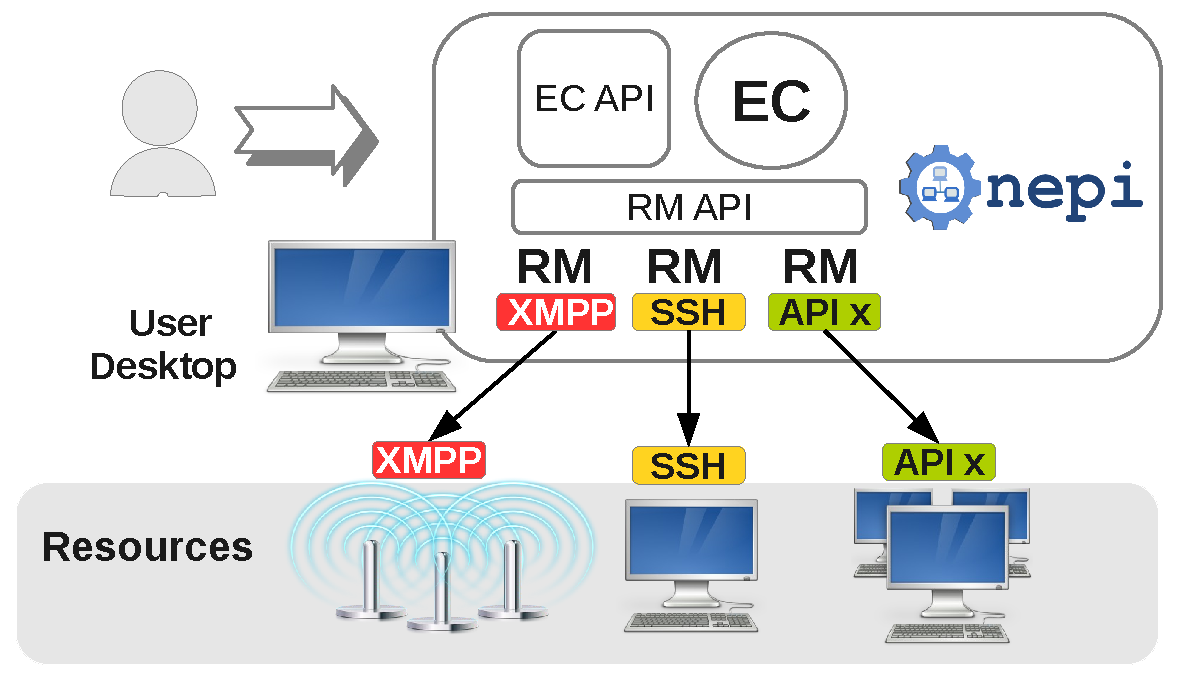
\includegraphics[width=\textwidth]{intro_resource_management}
  \caption{Resource management in NEPI}
  \label{fig:intro_resource_management}
\end{figure}


\chapter{The ExperimentController API}
\label{ec_api}
%%%%%%%%%%%%%%%%%%%%%%%%%%%%%%%%%%%%%%%%%%%%%%%%%%%%%%%%%%%%%%%%%%%%%%%%%%%%%%%
%
%    NEPI, a framework to manage network experiments
%    Copyright (C) 2013 INRIA
%
%    This program is free software: you can redistribute it and/or modify
%    it under the terms of the GNU General Public License as published by
%    the Free Software Foundation, either version 3 of the License, or
%    (at your option) any later version.
%
%    This program is distributed in the hope that it will be useful,
%    but WITHOUT ANY WARRANTY; without even the implied warranty of
%    MERCHANTABILITY or FITNESS FOR A PARTICULAR PURPOSE.  See the
%    GNU General Public License for more details.
%
%    You should have received a copy of the GNU General Public License
%    along with this program.  If not, see <http://www.gnu.org/licenses/>.
%
% Author: Alina Quereilhac <alina.quereilhac@inria.fr>
%
%%%%%%%%%%%%%%%%%%%%%%%%%%%%%%%%%%%%%%%%%%%%%%%%%%%%%%%%%%%%%%%%%%%%%%%%%%%%%%%


The ExperimentController (EC) is the entity in charge of turning the 
experiment description into a running experiment. 
In order to do this the EC needs to know which resources are to be 
used, how they should be configured and how resources relate to one another.
To this purpose the EC exposes methods to register resources, specify their 
configuration, and register dependencies between. These methods are part of
the EC design API.
Likewise, in order to deploy and control resources, and collect data, 
the EC exposes another set of methods, which form the execution API. 
These two APIs are described in detail in the rest of this chapter.


\section{The experiment script}

NEPI is a Python-based language and all classes and functions can
be used by importing the \emph{nepi} module from a Python script.

In particular, the ExperimentController class can be imported as follows:

\begin{lstlisting}[language=Python]

from nepi.execution.ec import ExperimentController

\end{lstlisting}

Once this is done, an ExperimentController must be instantiated for
the experiment. The ExperimentController constructor receives
the optional argument \emph{exp\_id}. This argument is important because
it defines the experiment identity and allows to distinguish among different
experiments. If an experiment id is not explicitly given, NEPI will automatically
generate a unique id for the experiment. 

\begin{lstlisting}[language=Python]

ec = ExperimentController(exp_id = "my-exp-id")

\end{lstlisting}

The experiment id can always be retrieved as follows

\begin{lstlisting}[language=Python]

exp_id = ec.exp_id 

\end{lstlisting}

Since a same experiment can be ran more than one time, and this is 
often desirable to obtain statistical data, the EC identifies 
different runs of an experiment with a same \emph{exp\_id} with  
another attribute, the \emph{run\_id}. The \emph{run\_id} is
a timestamp string value, and in combination with the \emph{exp\_id},
it allows to uniquely identify an experiment instance.

\begin{lstlisting}[language=Python]

run_id = ec.run_id 

\end{lstlisting}



\section{The design API}

Once an ExperimentController has been instantiated, it is possible to start
describing the experiment. The design API is the set of methods which
allow to do so.


\subsection{Registering resources}

Every resource supported by NEPI is controlled by a specific ResourceManager 
(RM). The RM instances are automatically created by the EC, and the user does 
not need to interact with them directly. 

Each type of RM is associated with a \emph{type\_id} which uniquely identifies 
a concrete kind of resource (e.g PlanetLab node, application that runs in
a Linux machine, etc).
The \emph{type\_ids} are string identifiers, and they are required  
to register a resource with the EC.

To discover all the available RMs and their \emph{type\_ids} we
can make use of the ResourceFactory class.
This class is a \emph{Singleton} that holds the templates and information 
of all the RMs supported by NEPI. We can retrieve this information as follows:

\begin{lstlisting}[language=Python]

from nepi.execution.resource import ResourceFactory

for type_id in ResourceFactory.resource_types():
    rm_type = ResourceFactory.get_resource_type(type_id)
    print type_id, ":", rm_type.get_help()

\end{lstlisting}

Once the \emph{type\_id} of the resource is known, the registration of a
new resource with the EC is simple:

\begin{lstlisting}[language=Python]

type_id = "SomeRMType"
guid = ec.register_resources(type_id)

\end{lstlisting}

When a resource is registered, the EC instantiates a RM of the 
requested \emph{type\_id} and assigns a global unique identifier 
(guid) to it. The guid is an incremental integer number and it 
is the value returned by the \emph{register\_resource} method.
The EC keeps internal references to all RMs, which the user can
reference using the corresponding guid value.


\subsection{Attributes}

ResourceManagers expose the configurable parameters of resources
through a list of attributes. An attribute can be seen as a
\emph{{name:value}} pair, that represents a certain aspect of
the resource (whether information or configuration information).

It is possible to discover the list of attributes exposed by an 
RM type as follows:

\begin{lstlisting}[language=Python]
from nepi.execution.resource import ResourceFactory

type_id = "SomeRMType"
rm_type = ResourceFactory.get_resource_type(type_id)

for attr in rm_type.get_attributes():
    print "       ",  attr.name, ":", attr.help
    
\end{lstlisting}

To configure or retrieve the value of a certain attribute of
an registered resource we can use the \emph{get} and \emph{set}
methods of the EC.

\begin{lstlisting}[language=Python]

old_value = ec.get(guid, "attr_name")
ec.set(guid, "attr_name", new_value)
new_value = ec.get(guid, "attr_name")

\end{lstlisting}

Since each RM type exposes the characteristics of a particular type
of resource, it is to be expected that different RMs will have different
attributes. However, there a particular attribute that is common to all RMs.
This is the \emph{critical} attribute, and it is meant to indicate to the EC
how it should behave when a failure occurs during the experiment. 
The \emph{critical} attribute has a default value of \emph{True}, since
all resources are considered critical by default. 
When this attribute is set to \emph{False} the EC will ignore failures on that 
resource and carry on with the experiment. Otherwise, the EC will immediately 
interrupt the experiment.


\subsection{Traces}

A Trace represent a stream of data collected during the experiment and associated
to a single resource. ResourceManagers expose a list of traces, which are identified
by a name. Particular traces might or might not need activation, since some traces
are enabled by default.

It is possible to discover the list of traces exposed by an 
RM type as follows:

\begin{lstlisting}[language=Python]
from nepi.execution.resource import ResourceFactory

type_id = "SomeRMType"
rm_type = ResourceFactory.get_resource_type(type_id)

for trace in rm_type.get_traces():
    print "       ",  trace.name, ":", trace.enabled
    
\end{lstlisting}

The \emph{enable\_trace} method allows to enable a specific trace for a 
RM instance

\begin{lstlisting}[language=Python]

ec.enable_trace(guid, "trace-name")

print ec.trace_enabled(guid, "trace-name")

\end{lstlisting}


\subsection{Registering connections}

In order to describe the experiment set-up, a resources need to be 
associated at least to one another. Through the process of connecting resources
the \emph{topology graph} is constructed. A certain application might
need to be configured and executed on a certain node, and this
must be indicated to the EC by connecting the application RM to the node
RM.

Connections are registered using the \emph{register\_connection} method,
which receives the guids of the two RM.

\begin{lstlisting}[language=Python]

ec.register_connection(node_guid, app_guid)

\end{lstlisting}

The order in which the guids are given is not important, since the
\emph{topology\_graph} is not directed, and the corresponding 
RMs \emph{`know'} internally how to interpret the connection 
relationship.


\subsection{Registering conditions}

All ResourceMangers must go through the same sequence of state transitions.
Associated to those states are the actions that trigger the transitions.
As an example, a RM will initially be in the state NEW. When the DEPLOY action
is invoked, it will transition to the DISCOVERED, then PROVISIONED, then READY
states. Likewise, the action START will make a RM pass from state READY to 
STARTED, and the action STOP will change a RM from state STARTED to STOPPED.

Using these states and actions, it is possible to specify workflow dependencies 
between resources. For instance, it would be possible to indicate that
one application should start after another application by registering a 
condition with the EC.

\begin{lstlisting}[language=Python]

from nepi.execution.resource import ResourceState, ResourceActions

ec.register_condition(app1_guid, ResourceAction.START, app2_guid, ResourceState.STARTED)

\end{lstlisting}

The above invocation should be read "Application 1 should START after application 2 
has STARTED". It is also possible to indicate a relative time from the moment a state
change occurs to the moment the action should be taken as follows:

\begin{lstlisting}[language=Python]

from nepi.execution.resource import ResourceState, ResourceActions

ec.register_condition(app1_guid, ResourceAction.START, app2_guid, ResourceState.STARTED, time = "5s")

\end{lstlisting}

This line should be read "Application 1 should START at least 5 seconds after 
application 2 has STARTED". \\

Allowed actions are: DEPLOY, START and STOP. \\

Existing states are: NEW, DISCOVERED, PROVISIONED, READY, STARTED, STOPPED, 
FAILED and RELEASED. \\



\section{The execution API}

After registering all the resources and connections and setting attributes and
traces, once the experiment we want to conduct has been described, we can
proceed to run it. To this purpose we make use of the \emph{execution} methods
exposed by the EC.


\subsection{Deploying an experiment}

Deploying an experiment is very easy, it only requires to invoke the 
\emph{deploy} method of the EC.

\begin{lstlisting}[language=Python]

ec.deploy()

\end{lstlisting}

Given the experiment description provided earlier, the EC will take care
of automatically performing all necessary actions to discover, provision,
configure and start all resources registered in the experiment. 

Furthermore, NEPI does not restrict deployment to only one time, it allows
to continue to register, connect and configure resources and deploy them
at any moment. We call this feature \emph{interactive} or \emph{dynamic}
deployment. 

The \emph{deploy} method can receive other optional arguments to customize
deployment. By default, the EC will deploy all registered RMs that are in
state NEW. However, it is possible to specify a subset of resources to be
deployed using the \emph{guids} argument.

\begin{lstlisting}[language=Python]

ec.deploy(guids=[guid1, guid2, guid3])

\end{lstlisting}

Another useful argument of the \emph{deploy} method is \emph{wait\_all\_ready}.
This argument has a default value of \emph{True}, and it is used as a barrier
to force the START action to be invoked on all RMs being deploy only after
they have all reached the state READY.

\begin{lstlisting}[language=Python]

ec.deploy(wait_all_ready=False)

\end{lstlisting}


\subsection{Getting attributes}

Attribute values can be retrieved at any moment during the experiment run, 
using the \emph{get} method. 
However, not all attributes can be modified after a resource has
been deployed. The possibility of changing the value of a certain attribute 
depends strongly on the RM and on the attribute itself. 
As an example, once a \emph{hostname} has been specified for a certain Node 
RM, it might not be possible to change it after deployment.

\begin{lstlisting}[language=Python]

attr_value = ec.get(guid, "attr-name")

\end{lstlisting}

Attributes have flags that indicate whether their values can be changed
and when it is possible to change them (e.g. before or after deployment, 
or both). These flags are \emph{NoFlags} (the attribute value can be 
modified always), \emph{ReadOnly} (the attribute value can never be
modified), \emph{ExecReadOnly} (the attribute value can only be modified
before deployment). The flags of a certain attribute can be validated 
as shown in the example below, and the value of the attribute can be
changed using the \emph{set} method.  

\begin{lstlisting}[language=Python]

from nepi.execution.attribute import Flags

attr = ec.get_attribute(guid, "attr-name")

if not attr.has_flag(Flags.ReadOnly):
    ec.set(guid, "attr-name", attr_value)

\end{lstlisting}

\subsection{Quering the state}

It is possible to query the state of any resource at any moment.
The state of a resource is requested using the \emph{state} method.
This method receives the optional parameter \emph{hr} to output the
state in a \emph{human readable} string format instead of an integer
state code.

\begin{lstlisting}[language=Python]

state_id = ec.state(guid)

# Human readable state
state = ec.state(guid, hr = True)

\end{lstlisting}

\subsection{Getting traces}

After a ResourceManager has been deployed it is possible to get information
about the active traces and the trace streams of the generated data using
the \emph{trace} method.

Most traces are collected to a file in the host where they are generated, 
the total trace size and the file path in the (remote) host can be 
retrieved as follows.

\begin{lstlisting}[language=Python]

from nepi.execution.trace import TraceAttr

path = ec.trace(guid, "trace-name", TraceAttr.PATH)
size = ec.trace(guid, "trace-name", TraceAttr.SIZE)

\end{lstlisting}

The trace content can be retrieved in a stream, block by block.

\begin{lstlisting}[language=Python]

trace_block = ec.trace(guid, "trace-name", TraceAttr.STREAM, block=1, offset=0)

\end{lstlisting}

It is also possible to directly retrieve the complete trace content.

\begin{lstlisting}[language=Python]

trace_stream = ec.trace(guid, "trace-name")

\end{lstlisting}

Using the \emph{trace} method it is easy to collect all traces 
to the local user machine. 

\begin{lstlisting}[language=Python]

for trace in ec.get_traces(guid):
    trace_stream = ec.trace(guid, "trace-name")
    f = open("trace-name", "w")
    f.write(trace_stream)
    f.close()

\end{lstlisting}


% TODO: how to retrieve an application trace when the Node failed? (critical attribute)


% \subsection{The collector RM}

%%%%%%%%%%
%% TODO
%%%%%%%%%%%

\subsection{API reference}

Further information about classes and method signatures
can be found using the Python \emph{help} method.
For this inspection work, we recommend to instantiate an
ExperimentController from an IPython console. This is an
interactive console that allows to dynamically send input
to the python interpreter. 

If NEPI is not installed in the system, you will need to add the
NEPI sources path to the PYTHONPATH environmental variable 
before invoking \emph{ipython}.

\begin{lstlisting}[language=Python]

$ PYTHONPATH=$PYTHONPATH:src ipython
Python 2.7.3 (default, Jan  2 2013, 13:56:14) 
Type "copyright", "credits" or "license" for more information.


IPython 0.13.1 -- An enhanced Interactive Python.
?         -> Introduction and overview of IPython's features.
%quickref -> Quick reference.
help      -> Python's own help system.
object?   -> Details about 'object', use 'object??' for extra details.

In [1]: from nepi.execution.ec import ExperimentController

In [2]: ec = ExperimentController(exp_id = "test-tap")

In [3]: help(ec.set)

\end{lstlisting}

The example above will show the following information related to the
\emph{set} method of the EC API.

\begin{lstlisting}[language=Python]

Help on method set in module nepi.execution.ec:

set(self, guid, name, value) method of nepi.execution.ec.ExperimentController instance
    Modifies the value of the attribute with name 'name' on the RM with guid 'guid'.
    
    :param guid: Guid of the RM
    :type guid: int
    
    :param name: Name of the attribute
    :type name: str
    
    :param value: Value of the attribute

\end{lstlisting}




\chapter{Supported resources}
\label{supported_resources}
%%%%%%%%%%%%%%%%%%%%%%%%%%%%%%%%%%%%%%%%%%%%%%%%%%%%%%%%%%%%%%%%%%%%%%%%%%%%%%%
%
%    NEPI, a framework to manage network experiments
%    Copyright (C) 2013 INRIA
%
%    This program is free software: you can redistribute it and/or modify
%    it under the terms of the GNU General Public License as published by
%    the Free Software Foundation, either version 3 of the License, or
%    (at your option) any later version.
%
%    This program is distributed in the hope that it will be useful,
%    but WITHOUT ANY WARRANTY; without even the implied warranty of
%    MERCHANTABILITY or FITNESS FOR A PARTICULAR PURPOSE.  See the
%    GNU General Public License for more details.
%
%    You should have received a copy of the GNU General Public License
%    along with this program.  If not, see <http://www.gnu.org/licenses/>.
%
% Author: Alina Quereilhac <alina.quereilhac@inria.fr>
%
%%%%%%%%%%%%%%%%%%%%%%%%%%%%%%%%%%%%%%%%%%%%%%%%%%%%%%%%%%%%%%%%%%%%%%%%%%%%%%%

\section{Linux resources}

\begin{itemize}
  \item Linux Node (Clean home, etc)
  \item SSH
  \item The directory structure
  \item Traces and collection
  \item Linux Application
  \item LinuxPing, LinuxTraceroute, etc
  \item CCNx
\end{itemize}

\section{Planetlab resources}

The Planetlab node resource inherits every feature of the Linux node, but adds the ability to choose for your experiment, healthy nodes from the Planetlab testbed. By healthy we mean alive nodes, accessible via ssh using your authentication information, with a checked filesystem in order to discard future problems during run-time.

\subsection{How to get an account}

  \subsubsection{Register}

If you want to use nodes from the Planetlab testbed, first you need to have an account, if you don't have one, you can register on the planetlab europe portal www.planet-lab.eu (see Create an account). 

  \subsubsection{Add your account to a Slice}

Then, in order to have access to the nodes needed for your experiment, you will need a slice. A slice is a subset of the planetlab resources, capable of running an experiment. Usually, once you own an account, you ask someone from your institue for a slice creation. The granted person ( called PI ) can then create a slice for you or associate you to an already existing slice.

  \subsubsection{Differences between PLE and PLC}

Different instamces of PlanetLab exist like PlanetLab Central, PlanetLab Europe, PlanetLab Japan,...  PlanetLab Europe (PLE) is the European portion of the publicly available PlanetLab (PLC) testbed. They main operational difference is related to credentials. If the testbed that issues the credentials is the european testbed, then for the PlanetLab Europe nodes the user can query more status information. Having more information can be beneficial when defining selection filters for the nodes. Anyway, PLE and PLC are federated, meaning the discovery and provisioning is always possible.

\subsection{The Planetlab Node RM}

In order for NEPI to select healthy nodes for your experiment and add them to your slice, it is necessary to set three attributes after resource registration : username, pluser and plpassword. username is the name to ssh login in your nodes, for Planetlab testbed it will always be your slice
name. pluser and plpassword are the user and password used for authenticate yourself in the Planetlab web page (www.planet-lab.eu). For example, when registering a Planetlab node for your experiment, the
experiment description will look a lot like this:
\begin{lstlisting}[language=Python]
node = ec.register_resource("planetlab::Node")
ec.set(node, "username", "institute_project")
ec.set(node, "pluser", "​​john.doe@institute.edu")
ec.set(node, "plpassword", "guessit")
\end{lstlisting}
When you log in with your credential to the Planetlab testbed portal (www.planet-lab.eu), you should be able to see the slices associated to your user as well as the set of nodes currently in your slices, and all the nodes provided by the testbed. Moreover, the web page allows the user to browse these resources and find out more characteristics about them. However, using the web site is not really convenient for large experiment involving hundreds of nodes. NEPI can do this job for you.

The portal retrieves the node's information by quering a service called MyPLC, NEPI queries the same service to efficiently select the most suitable nodes for the experiment. The user and password to query this service are the ones introduced before as pluser, and plpassword.

NEPI allows the user to filter among the Planetlab nodes according to different criterias, aiming to select a specific set of nodes for the experiment. For example, one experiment could only require nodes with OS Fedora 14, so the user should use the OS filter available for the Planetlab node resource when describing the node.

Current list of filters available :
\begin{itemize}
  \item city
  \item country
  \item region
  \item architecture
  \item operating\_system
  \item min\_reliability
  \item max\_reliability
  \item min\_bandwidth
  \item max\_bandwidth
  \item min\_load
  \item max\_load
  \item min\_cpu
  \item max\_cpu
\end{itemize}

We have already mentionned that, in order to use MyPLC service, it is necessary to set the attributes pluser and plpassword.  Filters are also represented by attributes and can be set by the user. Different type of filter exist, each one corresponding to a specific kind of value (String, Enumerate, ...). For each attribute, more information can be found in the help associated to this attribute as well as in its definition.

For example, for the attribute operating system, one can find the help, type, values allowed, etc. in its definition (src/nepi/resources/planetlab/node.py):
\begin{lstlisting}[language=Python]
operating_system = Attribute("operatingSystem", 
  "Constraint operating system during resource discovery.",
        type = Types.Enumerate,
        allowed = ["f8",
        "f12",
        "f14",
        "centos",
        "other"],
        flags = Flags.Filter)
\end{lstlisting}
Now we know how to add a filter to the node description:
\begin{lstlisting}[language=Python]
    node = ec.register_resource("planetlab::Node??")
    ec.set(node, "username", "institute_project")
    ec.set(node, "pluser", "​​jhon.doe@institute.edu")
    ec.set(node, "plpassword", "guessit")
    ec.set(node, "operatingSystem", "f14")
\end{lstlisting}
In case of more filters, an AND between the filters will be applied:

\begin{lstlisting}[language=Python]
    node = ec.register_resource("planetlab::Node??")
    ec.set(node, "username", "institute_project")
    ec.set(node, "pluser", "​​jhon.doe@institute.edu")
    ec.set(node, "plpassword", "guessit")
    ec.set(node, "operatingSystem", "f14")
    ec.set(node, "minCpu", 50)
\end{lstlisting}

Note that minCpu = 50 means that at least 50\% of the CPU has to be free in the node, to make the node suitable for the experiment.


\subsubsection{The hostname attribute}

Another attribute that the user can define for the node is the hostname. This attribute has priority over the others filters. When the experiment needs more than one node, it is necessary to register conditions in order to ensure that the nodes identified by its hostname are selected before the others nodes (the ones identified by filters or just not identified at all).

For example, imagine we need two nodes for our experiment :
Current list of filters available :
\begin{itemize}
  \item For one of them, we are completly sure that we want to use a specific one, so we identify it by its hostname
  \item For the other one, we just want to fulfill the restriction of OS fedora 8 and country France.
\end{itemize}

In this case, our experiment description will look like this:
\begin{lstlisting}[language=Python]
node1 = ec.register_resource("planetlab::Node")
ec.set(node1, "username", "institute_project")
ec.set(node1, "pluser", "​​john.doe@institute.edu")
ec.set(node1, "plpassword", "guessit")
ec.set(node1, "hostname", "planetlab2.utt.fr") 
## planetlab2.utt.fr is the specific node we want to use

node2 = ec.register_resource("planetlab::Node")
ec.set(node2, "username", "institute_project")
ec.set(node2, "pluser", "​​john.doe@institute.edu")
ec.set(node2, "plpassword", "guessit")
ec.set(node2, "operatingSystem", "f8")
ec.set(node2, "country", "France")
\end{lstlisting}
The nodes that are identified by their hostnames have to be provisioned before the rest of the nodes. This assures that no other resource will use the identified node even if the constraints matchs. Meaning that, even if the host "planetlab2.utt.fr" fulfills the conditions OS fedora 8 and country France, the node2 resource should not select from the planetlab testbed "planetlab2.utt.fr", the node1 must select it. We can enforce this to happen using the register\_condition method of the ec. Therefore, after registering the node and setting its attributes, we need to add this line:
\begin{lstlisting}[language=Python]
ec.register_condition(node2,ResourceAction.DEPLOY, node1, ResourceState.PROVISIONED)
\end{lstlisting}
For a better example on how to use filters and register conditions, there is the ping experiment example (examples/planetlab/ping\_experiment.py). In this example we define 5 nodes, and 4 ping applications running in 4 of the nodes, with the 5th one as destination. Then we collect the traces in our local machine.


\subsubsection{Persist blacklisted nodes}

PlanetLab nodes may fail for different reasons, ssh authentication failure, file system corrupted, nodes unreachable, between others. Moreover, the mal functioning nodes can vary from one experiment run to the next one. In NEPI there is the ability to register these mal functioning nodes in order run the experiment in a more efficient way. Also, this information can be use to evaluate the performance of the experiment and the nodes themselves.

The planetlab::Node resource, is instantiated for each Planetlab node defined in the experiment. The node discovery and provisioning occurs in parallel for every node defined, so a list of the nodes failures is needed while deploying, in order to avoid to repeat the provision of mal functioning nodes. This list of blacklisted nodes during the experiment, can be saved and maintain for following run of the same experiment or others experiments. This list it is called blacklist. Moreover, the nodes in the blacklist in the moment the experiment is started, can be use to directly discard from the node discover and provision the unwanted nodes.

There is an attribute available for this matter, is called 'persist\_blacklist' and is a global attribute, meaning that if set, is set for every resource of type planetlab::Node.
The blacklist file is stored in ~/.nepi/plblacklist.txt.

Example on how to use the attribute:

Two Planetlab nodes that read from the blacklist at the beginning of the experiment, and write new blacklisted nodes (if any) at the end.
\begin{lstlisting}[language=Python]
node1 = ec.register_resource("planetlab::Node")
ec.set(node1, "username", username)
ec.set(node1, "pluser", pl_user)
ec.set(node1, "plpassword", pl_password)
ec.set(node1, "cleanHome", True)
ec.set(node1, "cleanProcesses", True)

node2 = ec.register_resource("planetlab::Node")
ec.set(node2, "username", username)
ec.set(node2, "pluser", pl_user)
ec.set(node2, "plpassword", pl_password)
ec.set(node2, "cleanHome", True)
ec.set(node2, "cleanProcesses", True)

ec.set_global("planetlab::Node", 'persist_blacklist', True)
\end{lstlisting}
The attribute can be retrieved with the method get\_global :
\begin{lstlisting}[language=Python]
ec.get_global("planetlab::Node", 'persist_blacklist').
\end{lstlisting}
\subsection{SFA Support}

\subsubsection{Why using SFA for discovery and provision of resources in NEPI?}

In order to be able to reserve resources for cross testbed experiments without having to deal with different types of credentials, is important that testbed adopt the SFA interface and the users have at least one set of credentials in one testbed. With the SFA user credential, slice credential and authority credential, the user can list resources, allocate them, provision them, delete them from his slice, plus, add or remove slices when is allowed, in any SFA compliant testbed that trust each others registry. The last assures an uniform control plane operation layer (discovery, reservation, and provisioning) for every type of resource in any SFA compliant testbed.

NEPI developed the appropriate framework to be able to solve control plane operations through SFA. Based on the sfi client, NEPI developed an API that implement for the user, the corresponding SFA AM calls to handle the first steps of the experiment lifecycle. This is transparent for the user, who doesn't need to deal with SFA calls specifics, or understanding RSpecs (Resource specification). Moreover, NEPI implemented functions to assist in the selection of a set of reservable resources.

The use of SFA then, requires that the user installs the sfi client (version\_tag="3.1-4"), you can check http://svn.planet-lab.org/wiki/SFATutorial\#SFATutorial for more information. 

\subsubsection{SFA in PlanetLab}

This should not add complexity for the user, for example, for the Planetlab node, the experiment description is very similar:
\begin{lstlisting}[language=Python]
from nepi.execution.ec import ExperimentController
import os

# Create the EC
exp_id = "sfa_test"
ec = ExperimentController(exp_id)

username = os.environ.get('SFA_SLICE')  --- for example 'inria_lguevgeo'
sfauser = os.environ.get('SFA_USER')  --- for example 'ple.inria.lucia_guevgeozian_odizzio'
sfaPrivateKey = os.environ.get('SFA_PK')  --- for example '/home/.sfi/lucia_guevgeozian_odizzio.pkey'

node1 = ec.register_resource("planetlab::sfa::Node")
ec.set(node1, "hostname", 'planetlab1.cs.vu.nl')
ec.set(node1, "username", username)
ec.set(node1, "sfauser", sfauser)
ec.set(node1, "sfaPrivateKey", sfaPrivateKey)
ec.set(node1, "cleanHome", True)
ec.set(node1, "cleanProcesses", True)
\end{lstlisting}
\subsubsection{SFA with iMinds Testbed (w-iLab.t)}

The control and management software running in w-iLab.t is OMF 6, but its resources can be discover and provisioned using SFA, the experiment description for the WilabtSfaNode in NEPI is similar to the one in Planetlab::Node. Below is an example :
\begin{lstlisting}[language=Python]
from nepi.execution.ec import ExperimentController
import os

# Create the EC
exp_id = "sfa_test"
ec = ExperimentController(exp_id)

slicename = 'ple.inria.lguevgeo'
sfauser = os.environ.get('SFA_USER')
sfaPrivateKey = os.environ.get('SFA_PK')

# nodes
node1 = ec.register_resource("wilabt::sfa::Node")
ec.set(node1, "hostname", 'zotacM20')
ec.set(node1, "slicename", slicename)
ec.set(node1, "sfauser", sfauser)
ec.set(node1, "sfaPrivateKey", sfaPrivateKey)
ec.set(node1, "gatewayUser", "nepi")
ec.set(node1, "gateway", "bastion.test.iminds.be")
ec.set(node1, "cleanHome", True)
ec.set(node1, "cleanProcesses", True)
\end{lstlisting}

Note that the w-iLab.t testbed is a private testbed, and resources can be accessed only through a gateway. The node description must have two attributes defined as gatewayUser and gateway. The appropriate ssh key settings in the gateway must be pre-arranged with the testbed administrators, in order to enable the ssh access.

The gateway feature is not only possible for the w-iLab.t testbed, but for any testbed that allow ssh key authentication. The ability to store the blacklisted nodes is also possible for the w-iLab.t testbed.




\subsection{The vsys system}
    TO DO

  \subsubsection{Python Vsys}
    TO DO

  \subsubsection{TAP/TUN/TUNNEL}
    TO DO




\section{OMF resources}

This section aims at providing some information about OMF and its implementation in NEPI. Regarding to OMF itself, this user manual is not the official OMF Documenation and must be considered only as a complement to the official one (https://mytestbed.net/), gathering information collected during few years working with OMF.

\subsection{OMF 5.4 vs OMF 6}

Two versions really different of OMF exists and are already deployed in different testbed. OMF 5.4.x is the oldest one and is not anymore under development. Many testbed use this version in their testbed and start step by step to migrate towards OMF 6. This latter is still under development. Some projects, as Fed4Fire, want to use this technology and put many efforts to deploy this new version. 

Among the main differences between these two versions, we can noticed :
\begin{itemize}
\item OMF 5.4 use a Resource Controller (RC) that handles messages received throught XMPP. OMF 6 use a Resource Proxy (RP) that allow the posibility to create a Resource Controller to control an entity. So There is only one RP but one RC for each entity involved in the experiment.
\item The message protocol in OMF 5.4 use some specific keywords to create action, or configure data. It is not really flexible and was not prepared for extension. In OMF6, the protocol is well-defined and highly thought to be extensible as mush as possible. It is base on 5 routines that allow any action. This protocol is called FRCP.
\item Both of them use OEDL as description language. 
\end{itemize}

\subsection{Available OMF Testbed}

This subsection gather some information about well-known OMF Testbed. This list is not exhaustive and many others OMF-testbeds are under deployment.

\subsubsection{Nicta Testbed : Norbit}

Nicta is the main developers institute of OMF. It has also its own testbed, called Norbit, containing around 40 nodes deployed on a building. These nodes are usually ALIX nodes, with small power consumption and CPU performance. 
More details can be found on their website : 
http://mytestbed.net/projects/1/wiki/OMFatNICTA

\subsubsection{Nitos Testbed : NitLab}

Nitos is deployed in Greece on a 4th, 5th and 6th floor of a building in the city. Different nodes are deployed as commell or diskless node, but some new powerful nodes will be deployed soon, called Icarus Node, with high CPU performance. The total number of nodes deployed on this testbed is around 50.

More details can be found on their website : 
http://nitlab.inf.uth.gr/NITlab/

\subsubsection{iMinds Testbed : W-ilab.t}

iMinds is deployed in Belgium. The W-ilab.t testbed gather more that one testbed. Among them, there is one in Zwijnaarde that use OMF. Around 60 nodes are deployed on the ceil of their building and one room is reserved for mobile nodes ( using Roomba ). Around 10 mobile nodes will be deployed and operationnal in 2014.

More details can be found on their website : 
http://www.crew-project.eu/portal/wilab/basic-tutorial-your-first-experiment-w-ilabt

\subsection{How to get an Account}

Usually, the creation of the account need to be asked by email. Specific instructions are provided below about how to request an account : 
\begin{itemize}
\item Nicta : Ask thierry.rakotoarivelo@nicta.com.au 
\item Nitos : Use your onelab account (if you already have one) or create a new account directly on their website 
( http://nitlab.inf.uth.gr/NITlab/index.php/testbed )
\item iMinds : You need a VPN access and a Testbed Account. For the VPN Account, ask stefan.bouckaert@iminds.be and check the tips below to install OpenVPN. For the Testbed Account, ask pieter.becue@intec.ugent.be or directly on the w-iLabt.t web interface (It will required the VPN Access)
\end{itemize}

\subsubsection{Tips about OpenVPN}

To install OpenVPN from the sources, be sure that lib-lzo and lib-ssl are installed. If not, ./configure will allow to disable it by doing --disable-lzo or --disable-crypto. You should NOT do it unless you know what you are doing.
To install the components, follow these commands :
\begin{itemize}
\item For Lzo : 
\begin{itemize}
\item sudo apt-get install liblzo2-2 liblzo2-dev 
\item OR from the ​source (http://www.oberhumer.com/opensource/lzo/\#download) following these instructions 
(http://www.linuxfromscratch.org/blfs/view/6.3/general/LZO.html)
\end{itemize}
\item For Openssl : sudo apt-get install libssl-dev 
\end{itemize}
Finally, You will have to launch OpenVPN using the credentials you received from the testbed owner. The command will be something like :
sudo openvpn file.ovpn

\subsection{How to reserve some nodes}

After creating your account, you need to reserve some nodes to deploy your experiment on them. Different policies are used until now but it will move toward a common policy called Broker. 

This is the list of the current reservation method :
\begin{itemize}
\item Nicta : Use google calendar for a gentleman's agreement. Add your reservations directly in the google calendar. This functionality is enable only after asking the Nicta team to add your Gmail address.
\item Nitos : While logged into the website, you can use the Nitos ​Scheduler to reserve some nodes and some channels for a maximum period of 4hours
\item iMinds : Reserve your experiment on their website 
http://boss.wilab2.ilabt.iminds.be/reservation/. Your experiment should be swapped in automatically. If it is not the case, turn on your experiment on their website 
(https://www.wilab2.ilabt.iminds.be/) and the provisionning will be done by their tools. The number of nodes you required through the interfaces will be allocated for you with the image you declare (default image is Ubuntu 12.04 if nothing has been specified)
\end{itemize}


\subsection{XMPP}

The default communication layer used in OMF is XMPP. Xmpp is a PubSub communication system based on group. A group respresent a set of resource that can subscribe to this group. Each resource can then publish to this group and consequently send some messages to each resource that also subscribed.
Even if AMQP is supported by OMF, NEPI support only XMPP as it is mainly deployed on all the testbed.

The implementation of the XMPP client is based on the library SleekXmpp. Each method has been overwritten to fit the requirement we need to OMF. 

Finally, There is an OMF XMPP Factory that allow for each OMF Resource Manager to share the same Xmpp Client. Based on some credentials as the user or the password, the OMF XMPP factory store the different XMPP Client. When an OMF RM wants to communicate, it ask the Factory to retrieve one XMPP Client using the credentials it has or to create one if it doesn't exists. The factory store the number of RM that use each XMPP Client and delete it when no RM use it.












%%\chapter{ExperimentController internals}
%%\label{ec_internals}
%%%%%%%%%%%%%%%%%%%%%%%%%%%%%%%%%%%%%%%%%%%%%%%%%%%%%%%%%%%%%%%%%%%%%%%%%%%%%%%%%
%
%    NEPI, a framework to manage network experiments
%    Copyright (C) 2013 INRIA
%
%    This program is free software: you can redistribute it and/or modify
%    it under the terms of the GNU General Public License as published by
%    the Free Software Foundation, either version 3 of the License, or
%    (at your option) any later version.
%
%    This program is distributed in the hope that it will be useful,
%    but WITHOUT ANY WARRANTY; without even the implied warranty of
%    MERCHANTABILITY or FITNESS FOR A PARTICULAR PURPOSE.  See the
%    GNU General Public License for more details.
%
%    You should have received a copy of the GNU General Public License
%    along with this program.  If not, see <http://www.gnu.org/licenses/>.
%
% Author: Alina Quereilhac <alina.quereilhac@inria.fr>
%
%%%%%%%%%%%%%%%%%%%%%%%%%%%%%%%%%%%%%%%%%%%%%%%%%%%%%%%%%%%%%%%%%%%%%%%%%%%%%%%

% ExperimentController internals

\begin{itemize}
    \item the RMs dictionary
    \item The scheduling API
    \item The scheduler queue, the tasks dictionary, the schedule method 
    \item the processing thread and the \_process method, the inmediate execution queueu and the ParallelRunner
    \item the \_execute method 
    \item The deploy method (implementation), deployment groups
    \item The FailManager and what happens upon release (critical attribute)
\end{itemize}


%%\chapter{ResourceManager internals}
%%\label{rm_internals}
%%%%%%%%%%%%%%%%%%%%%%%%%%%%%%%%%%%%%%%%%%%%%%%%%%%%%%%%%%%%%%%%%%%%%%%%%%%%%%%%%
%
%    NEPI, a framework to manage network experiments
%    Copyright (C) 2013 INRIA
%
%    This program is free software: you can redistribute it and/or modify
%    it under the terms of the GNU General Public License as published by
%    the Free Software Foundation, either version 3 of the License, or
%    (at your option) any later version.
%
%    This program is distributed in the hope that it will be useful,
%    but WITHOUT ANY WARRANTY; without even the implied warranty of
%    MERCHANTABILITY or FITNESS FOR A PARTICULAR PURPOSE.  See the
%    GNU General Public License for more details.
%
%    You should have received a copy of the GNU General Public License
%    along with this program.  If not, see <http://www.gnu.org/licenses/>.
%
% Author: Alina Quereilhac <alina.quereilhac@inria.fr>
%
%%%%%%%%%%%%%%%%%%%%%%%%%%%%%%%%%%%%%%%%%%%%%%%%%%%%%%%%%%%%%%%%%%%%%%%%%%%%%%%

%ResourceManger internals

\begin{itemize}
  \item States
  \item Actions
  \item RM API (the schedule methods and the internal methods do\_blah, the states and times are recorded)
  \item failtrap
  \item RM inheritance
  \item init\_copy
  \item Adding new attributes
  \item Traces and the trace method
  \item The start\_with\_condition method and the conditions structure 
  \item How to enforce internal conditions by re-scheduling
\end{itemize}



%%\chapter{Extending NEPI: The CCNx case}
%%\label{extending_nepi}
%%%%%%%%%%%%%%%%%%%%%%%%%%%%%%%%%%%%%%%%%%%%%%%%%%%%%%%%%%%%%%%%%%%%%%%%%%%%%%%%%
%
%    NEPI, a framework to manage network experiments
%    Copyright (C) 2013 INRIA
%
%    This program is free software: you can redistribute it and/or modify
%    it under the terms of the GNU General Public License as published by
%    the Free Software Foundation, either version 3 of the License, or
%    (at your option) any later version.
%
%    This program is distributed in the hope that it will be useful,
%    but WITHOUT ANY WARRANTY; without even the implied warranty of
%    MERCHANTABILITY or FITNESS FOR A PARTICULAR PURPOSE.  See the
%    GNU General Public License for more details.
%
%    You should have received a copy of the GNU General Public License
%    along with this program.  If not, see <http://www.gnu.org/licenses/>.
%
% Author: Alina Quereilhac <alina.quereilhac@inria.fr>
%
%%%%%%%%%%%%%%%%%%%%%%%%%%%%%%%%%%%%%%%%%%%%%%%%%%%%%%%%%%%%%%%%%%%%%%%%%%%%%%%

TODO



\chapter{Debbuging}
\label{debugging}
%%%%%%%%%%%%%%%%%%%%%%%%%%%%%%%%%%%%%%%%%%%%%%%%%%%%%%%%%%%%%%%%%%%%%%%%%%%%%%%
%
%    NEPI, a framework to manage network experiments
%    Copyright (C) 2013 INRIA
%
%    This program is free software: you can redistribute it and/or modify
%    it under the terms of the GNU General Public License as published by
%    the Free Software Foundation, either version 3 of the License, or
%    (at your option) any later version.
%
%    This program is distributed in the hope that it will be useful,
%    but WITHOUT ANY WARRANTY; without even the implied warranty of
%    MERCHANTABILITY or FITNESS FOR A PARTICULAR PURPOSE.  See the
%    GNU General Public License for more details.
%
%    You should have received a copy of the GNU General Public License
%    along with this program.  If not, see <http://www.gnu.org/licenses/>.
%
% Author: Alina Quereilhac <alina.quereilhac@inria.fr>
%
%%%%%%%%%%%%%%%%%%%%%%%%%%%%%%%%%%%%%%%%%%%%%%%%%%%%%%%%%%%%%%%%%%%%%%%%%%%%%%%

TODO


%%\chapter{Unit testing}
%%\label{unit_testing}
%%%%%%%%%%%%%%%%%%%%%%%%%%%%%%%%%%%%%%%%%%%%%%%%%%%%%%%%%%%%%%%%%%%%%%%%%%%%%%%%%
%
%    NEPI, a framework to manage network experiments
%    Copyright (C) 2013 INRIA
%
%    This program is free software: you can redistribute it and/or modify
%    it under the terms of the GNU General Public License as published by
%    the Free Software Foundation, either version 3 of the License, or
%    (at your option) any later version.
%
%    This program is distributed in the hope that it will be useful,
%    but WITHOUT ANY WARRANTY; without even the implied warranty of
%    MERCHANTABILITY or FITNESS FOR A PARTICULAR PURPOSE.  See the
%    GNU General Public License for more details.
%
%    You should have received a copy of the GNU General Public License
%    along with this program.  If not, see <http://www.gnu.org/licenses/>.
%
% Author: Alina Quereilhac <alina.quereilhac@inria.fr>
%
%%%%%%%%%%%%%%%%%%%%%%%%%%%%%%%%%%%%%%%%%%%%%%%%%%%%%%%%%%%%%%%%%%%%%%%%%%%%%%%

TODO


\chapter{Release Cycle}
\label{release_cycle}
%%%%%%%%%%%%%%%%%%%%%%%%%%%%%%%%%%%%%%%%%%%%%%%%%%%%%%%%%%%%%%%%%%%%%%%%%%%%%%%
%
%    NEPI, a framework to manage network experiments
%    Copyright (C) 2013 INRIA
%
%    This program is free software: you can redistribute it and/or modify
%    it under the terms of the GNU General Public License as published by
%    the Free Software Foundation, either version 3 of the License, or
%    (at your option) any later version.
%
%    This program is distributed in the hope that it will be useful,
%    but WITHOUT ANY WARRANTY; without even the implied warranty of
%    MERCHANTABILITY or FITNESS FOR A PARTICULAR PURPOSE.  See the
%    GNU General Public License for more details.
%
%    You should have received a copy of the GNU General Public License
%    along with this program.  If not, see <http://www.gnu.org/licenses/>.
%
% Author: Alina Quereilhac <alina.quereilhac@inria.fr>
%
%%%%%%%%%%%%%%%%%%%%%%%%%%%%%%%%%%%%%%%%%%%%%%%%%%%%%%%%%%%%%%%%%%%%%%%%%%%%%%%

Releases in NEPI do not occur in strictly regular periods. Usually a new
release will be done every 4 or 5 months.

\section{The development branch}

The main development branch for NEPI 3 is \emph{nepi-3-dev}. 
There might be other branches to develop new features, but they will 
eventually end up being merged into the \emph{nepi-3-dev} branch. 

\section{Versioning}

Releases are named following the \emph{major.minor.revision} convention.
The \emph{major} number reflects a major change in functionality or architecture. 
It is to be expected that this number will remind in 3 for a long period.

The \emph{minor} number reflects the incorporation of new features into NEPI.
This number is expected to be increased on each release.

The \emph{revision} number is incremented when a considerable number of
bugs have been fixed. No release will be done when only the \emph{revision}
number is incremented.

\section{The release process}

The creation of a new NEPI release will always follow the same sequence of steps.

\begin{enumerate}
  \item A new \emph{nepi-3.<minor>-pre-release} branch will be created from the \emph{nepi-3-dev} branch
  \item During two to three weeks intensive work on testing will be carried out on the new branch. No new functionality will be added on this branch and only changes that fix bugs will be accepted.
  \item At the end of this period, the pre-release branch will be branched again into the release branch, named \emph{nepi-3.<minor>-release}
  \item A tag will be added to this new branch including the revision number (i.e. \emph{release-3.<minor>.<revision>})
  \item Finally, the pre-release branch will be merged into the development branch, nepi-3-dev, to incorporate to it all the bug fixes.
\end{enumerate}

%%TODO: Explain how to create patch



%%\chapter{Coding Style}
%%\label{coding_style}
%%%%%%%%%%%%%%%%%%%%%%%%%%%%%%%%%%%%%%%%%%%%%%%%%%%%%%%%%%%%%%%%%%%%%%%%%%%%%%%%%
%
%    NEPI, a framework to manage network experiments
%    Copyright (C) 2013 INRIA
%
%    This program is free software: you can redistribute it and/or modify
%    it under the terms of the GNU General Public License as published by
%    the Free Software Foundation, either version 3 of the License, or
%    (at your option) any later version.
%
%    This program is distributed in the hope that it will be useful,
%    but WITHOUT ANY WARRANTY; without even the implied warranty of
%    MERCHANTABILITY or FITNESS FOR A PARTICULAR PURPOSE.  See the
%    GNU General Public License for more details.
%
%    You should have received a copy of the GNU General Public License
%    along with this program.  If not, see <http://www.gnu.org/licenses/>.
%
% Author: Alina Quereilhac <alina.quereilhac@inria.fr>
%
%%%%%%%%%%%%%%%%%%%%%%%%%%%%%%%%%%%%%%%%%%%%%%%%%%%%%%%%%%%%%%%%%%%%%%%%%%%%%%%

TODO


\end{document}
